\chapter{Motivation}
There is current theoretical and experimental interest in a massive $U(1)$ vector boson that does not couple directly to particles in the Standard Model, but gains a weak effective coupling to charged particles through kinetic mixing.
This particle is commonly called a heavy photon, dark photon, or $A'$, and is characterized by its mass $m_{A'}$ and a dimensionless coupling constant $\epsilon$.

The heavy photon is primarily motivated as part of a larger ``dark sector'' of particles that are not charged directly under the Standard Model forces.
Some sort of ``portal'' is necessary to create an interaction between the dark sector and the Standard Model.
The possible portals are restricted by the symmetries of the Standard Model, and the dominant candidates are commonly referred to as the vector, Higgs, neutrino, and axion portals; the heavy photon is the mediator for the vector portal \cite{essig_dark_2013}.
Dark sector particles are natural candidates for dark matter, and a heavy photon can be part of a mechanism that produces the observed dark matter abundance.

%Massive U(1) vector bosons, also known as heavy photons, are a natural consequence of many theories of physics beyond the Standard Model.
%Such a particle could kinetically mix with the photon, giving it an effective coupling to electric charge much smaller than the photon's direct coupling $\alpha$.
%A heavy photon is one of several ``portals'' by which a dark sector could interact with Standard Model matter.
%
%The existence of such a heavy photon is a possible explanation for the cosmic ray positron excess and the muon $g-2$ anomaly.

\section{Theory Summary}
The basic assumption behind the heavy photon is that there exists a second (broken) $U(1)$ symmetry, and that it interacts with Standard Model hypercharge via kinetic mixing \cite{holdom_two_1986}.
At low energies, this leads to the following gauge field Lagrangian, where $F_{\mu\nu}=\partial_\mu A_\nu - \partial_\nu A_\mu$ is the electromagnetic field strength, $F'_{\mu\nu} = \partial_\mu A'_\nu - \partial_\nu A'_\mu$ is the heavy photon field strength, and $\epsilon$ is the dimensionless coupling constant:

\begin{equation}
    \mathcal{L}_{\mathrm{gauge}}=-\frac{1}{4}F^{\mu\nu}F_{\mu\nu} - \frac{1}{4}F'^{\mu\nu}F'_{\mu\nu} + \frac{1}{2}\epsilon F^{\mu\nu}F'_{\mu\nu}
\end{equation}

The kinetic mixing means that the fields are not orthogonal.
Orthogonality can be restored by redefining the electromagnetic field according to $A^\mu \to A^\mu + \epsilon A'^\mu$.
This modifies the interaction Lagrangian as follows:

\begin{equation}
    A^\mu J^{EM}_\mu \to A^\mu J^{EM}_\mu + \epsilon A'^\mu J^{EM}_\mu 
\end{equation}

This implies that particles with electric charge acquire a coupling, proportional to $\epsilon$, to the heavy photon.
%The converse is not true: hidden-sector particles with heavy photon couplings do not acquire couplings to the photon (such ``millicharged'' particles do occur if the new $U(1)$ is unbroken \cite{prinz_search_1998,davidson_updated_2000}) \cite{holdom_two_1986}.

If particles exist that are charged under both fields, kinetic mixing may arise from a one-loop diagram similar to Figure \ref{fig:oneloop}, with a natural scale of $\epsilon \sim 10^{-2}-10^{-4}$; on the other hand, GUT models require that one-loop contributions to $\epsilon$ vanish, and instead motivate two-loop contributions at $\epsilon \sim 10^{-3}-10^{-6}$ \cite{arkani-hamed_lhc_2008}.
Because kinetic mixing is a renormalizable interaction, $\epsilon$ is independent of the masses of the particles that give rise to it.
String theory models can motivate much smaller $\epsilon$, as low as $10^{-12}$ \cite{goodsell_naturally_2009,cicoli_testing_2011}.

\begin{figure}[ht]
    \begin{center}
        \begin{fmffile}{oneloop}
            \begin{fmfgraph*}(150,150)
                \fmfstraight 
                \fmfleft{i1}
                \fmfright{o1}
                \fmflabel{$\gamma$}{i1}
                \fmflabel{$A'$}{o1}
                \fmf{photon,tension=2}{i1,v1}
                \fmf{photon,tension=2}{v2,o1}
                \fmf{fermion,left}{v1,v2}
                \fmf{fermion,left}{v2,v1}
            \end{fmfgraph*}
        \end{fmffile}
    \end{center}
    \caption{One-loop diagram leading to kinetic mixing.}
    \label{fig:oneloop}
\end{figure}

There is a wide range of reasonable values for the mass $m_{A'}$.
Models where supersymmetry breaking is communicated by the kinetic mixing lead to natural mass scales of MeV-GeV \cite{baumgart_non-abelian_2009, morrissey_abelian_2009, cheung_kinetic_2009}.
String theory models typically tie the mass scale to $\epsilon$, and can motivate masses down to the meV scale \cite{goodsell_naturally_2009,cicoli_testing_2011}.

%If the new $U(1)$ is massless, the photon can be
%If the $A'$ is massless, the new $U(1)$ mixes 
%particles charged under the $A'$ gain a small electromagnetic charge. 
%
%Such millicharged particles have been the subject of direct experimental searches


%If the $A'$ is massive, particles charged under the $A'$ do not 
%
%massless U(1)': millicharge, paraphoton
%paraphoton doesn't couple to normal matter, para-matter gets millicharged
%
%massive U(1)': heavy photon
%photon doesn't couple to hidden sector, heavy photon couples to SM matter

\section{Observations Motivating a Heavy Photon}

\subsection{Dark Matter Annihilation}

Dark matter annihilation mediated by a heavy photon has been proposed as an explanation for several anomalies that have been reported in cosmic ray and X-ray observations.

The PAMELA satellite first observed that the positron fraction $\phi(e^+)/(\phi(e^+)+\phi(e^-))$ increases above 10 GeV.
This is inconsistent with the assumption that high-energy positrons originate in secondary production processes, from cosmic-ray nuclei interactions with interstellar gas.
Meanwhile, the antiproton fraction is consistent with secondary production.
Measurements by the Fermi Large Area Telescope and the Alpha Magnetic Spectrometer (AMS) confirmed the observation and extended it to higher energies \cite{the_fermi_lat_collaboration_measurement_2012,ams_collaboration_first_2013}.

The annihilation cross-section implied by the positron flux is large compared to the cross-section expected for a thermal relic, and also much larger than any observed annihilation to hadrons \cite{cholis_high_2009}.
This is consistent with annihilation to heavy photons which then decay to electrons and positrons, as shown in Figure \ref{fig:dm_annihilation} \cite{arkani-hamed_theory_2009}.
A heavy photon with $m_{A'}<2m_p$ cannot decay to $p\bar{p}$, and $m_{A'}$ in the MeV--GeV range (models with $m_{A'}$ in the 200--900 MeV range were tested in \cite{finkbeiner_consistent_2011}; if annihilation is dominated by local subhalos, lower mass ranges are allowed \cite{slatyer_sommerfeld-enhanced_2012}) creates Sommerfeld enhancement that boosts the annihilation cross-section at low velocities.

\begin{figure}[ht]
    \begin{center}
        \begin{fmffile}{annihilation}
            \begin{fmfgraph*}(150,150)
                \fmfstraight 
                \fmfleft{i1,i2}
                \fmfright{o0,o1,o2,o3}
                \fmflabel{$\chi$}{i1}
                \fmflabel{$\chi$}{i2}
                \fmflabel{$A'$}{o1}
                \fmflabel{$A'$}{o2}
                \fmf{fermion}{i1,v1,v2,i2}
                \fmf{photon}{v1,o1}
                \fmf{photon}{v2,o2}
                %\fmf{fermion}{o1,v3,o2}
                %\fmf{fermion}{o3,v4,o4}
            \end{fmfgraph*}
        \end{fmffile}
    \end{center}
    \caption{Dark matter annihilation to a heavy photon, which can then decay to Standard Model particles.}
    \label{fig:dm_annihilation}
\end{figure}

The positron fraction has more recently been disfavored as a motivation for the heavy photon.
A larger AMS data set shows the full shape of the positron spectrum is softer than would be expected from a heavy photon decaying directly to $e^+e^-$ \cite{ams_collaboration_high_2014}, but consistent with a pulsar origin for cosmic ray positrons \cite{cholis_dark_2013}.
Meanwhile, CMB observations put limits on the DM annihilation rate at recombination; measurements by Planck severely limit the DM annihilation explanation for the positron fraction \cite{madhavacheril_current_2014}.
The positron spectrum may still be consistent with heavy photons decaying to intermediate states that then decay to $e^+e^-$ \cite{cholis_dark_2013}.

Gamma ray and X-ray excesses also motivate models of dark matter that include heavy photons.
Dark matter annihilation has been proposed as a source for an excess of high-energy gamma rays from the Galactic Center in Fermi data, and hidden sectors can play a role \cite{hooper_dark_2011}.
A 3.5 keV line seen in galaxy cluster X-ray spectra \cite{bulbul_detection_2014,boyarsky_unidentified_2014} has been suggested to come from collisional excitation and de-excitation of dark matter, in a model named eXciting Dark Matter (XDM) \cite{finkbeiner_x-ray_2014}.

\subsection{Halo Structure}
Observations of dark matter halos of galaxies and dwarf galaxies disagree with predictions based on the assumption of collisionless cold dark matter \cite{weinberg_cold_2013}.
These discrepancies have motivated models (``self-interacting dark matter,'' or SIDM) in which dark matter is self-interacting with a large but velocity-dependent cross-section, consistent with a heavy photon mediator.
This allows momentum diffusion in halos without disrupting high-velocity events such as the Bullet Cluster \cite{spergel_observational_2000,tulin_beyond_2013}.

Rotational velocities of observed Milky Way dwarf satellite galaxies are lower than the rotational velocities that simulations predict for the Milky Way's largest dark matter subhaloes.
This suggests that either the most massive dark matter subhalos fail to form dwarf galaxies, the massive subhalos do not exist, or the rotational velocities for a given subhalo mass are lower than predicted; this is known as the ``too big to fail'' problem \cite{boylan-kolchin_too_2011}.
Self-interacting dark matter reduces the central densities of subhalos and thus the rotational velocities \cite{vogelsberger_subhaloes_2012}.
Similarly, the observed density profiles of galaxies are better fit with a constant density core than the cuspy models from collisionless dark matter: this is the ``cusp-core'' problem \cite{de_naray_baryons_2011}
Both the observational evidence and the simulations continue to develop, and it may be possible to resolve the conflicts without abandoning collisionless dark matter \cite{oman_unexpected_2015,governato_cuspy_2012}.

%\subsection{Light Dark Matter}

\subsection{Muon $g-2$ Anomaly}
The measured value of the muon $g-2$ (anomalous magnetic moment, also known as $a_\mu=(g-2)/2$) is more than 3 standard deviations away from the value predicted by the Standard Model \cite{muon_final_2006,blum_muon_2013}.
A heavy photon can contribute to the magnetic moment through the diagram shown in Figure \ref{fig:gm2}; there is a specific band in the $\epsilon-m_{A'}$ parameter space (shown in green in Figure \ref{fig:reach}) where the heavy photon correction accounts for the anomaly \cite{pospelov_secluded_2009-1}.
The good agreement of the electron $g-2$ with the Standard Model excludes a different region (drawn in red); similarly, there is an excluded region (drawn in green, above the favored band) where the heavy photon correction to muon $g-2$ exceeds the observed anomaly \cite{endo_constraints_2012}.
This favored region has been targeted by many experiments, and is now excluded for the case of heavy photon decays to visible particles.

\begin{figure}[ht]
    \begin{center}
        \begin{fmffile}{gm2}
            \begin{fmfgraph*}(150,150)
                \fmfstraight 
                \fmftop{o1}
                \fmfbottom{i1,i2}
                \fmflabel{$\mu$}{i1}
                \fmflabel{$\mu$}{i2}
                \fmf{fermion}{i1,v1,v2,v3,i2}
                \fmf{photon,label=$\gamma$}{v2,o1}
                \fmffreeze
                \fmf{photon,label=$A'$}{v1,v3}
            \end{fmfgraph*}
        \end{fmffile}
    \end{center}
    \caption{Heavy photon correction to the muon magnetic moment.}
    \label{fig:gm2}
\end{figure}


\section{Signatures}
\label{sec:signatures}

The heavy photon's only coupling to the Standard Model is through kinetic mixing with the photon.
So assuming that heavy photon decays to the dark sector are kinematically forbidden, the production and decay of a heavy photon are closely related to the production and decay of a virtual photon with the same mass.

The branching fractions for decay, as a function of $m_{A'}$, can be derived from the ratios of cross sections for different final states of $e^+e^-$ collisions, as a function of center-of-mass energy: see Figure \ref{fig:branching}.
The decay width and proper lifetime are given in Equations \ref{eq:width} and \ref{eq:lifetime}, where $N_{eff}$ is the effective number of possible available decay products: neglecting phase-space corrections, $N_{eff}=1$ for $m_{A'}<2m_\mu$, and $N_{eff}=2+R(m_{A'})$ for $m_{A'}\ge 2m_\mu$, where $R(Q)=\frac{\sigma(e^+e^-\to \mathrm{hadrons},Q)}{\sigma(e^+e^-\to \mu^+\mu^-,Q)}$.

\begin{equation}
    \Gamma = \frac{N_{eff}m_{A'} \alpha \epsilon^2}{3}
    \label{eq:width}
\end{equation}

\begin{equation}
    \tau = \frac{\hbar}{\Gamma} = \frac{3\hbar}{N_{eff}m_{A'} \alpha \epsilon^2}
    \label{eq:lifetime}
\end{equation}

Since $\epsilon^2$ is small, the decay width is very narrow ($\Gamma/m_{A'}\propto \alpha \epsilon^2$) and the heavy photon appears as a sharp resonance.

\begin{figure}[ht]
    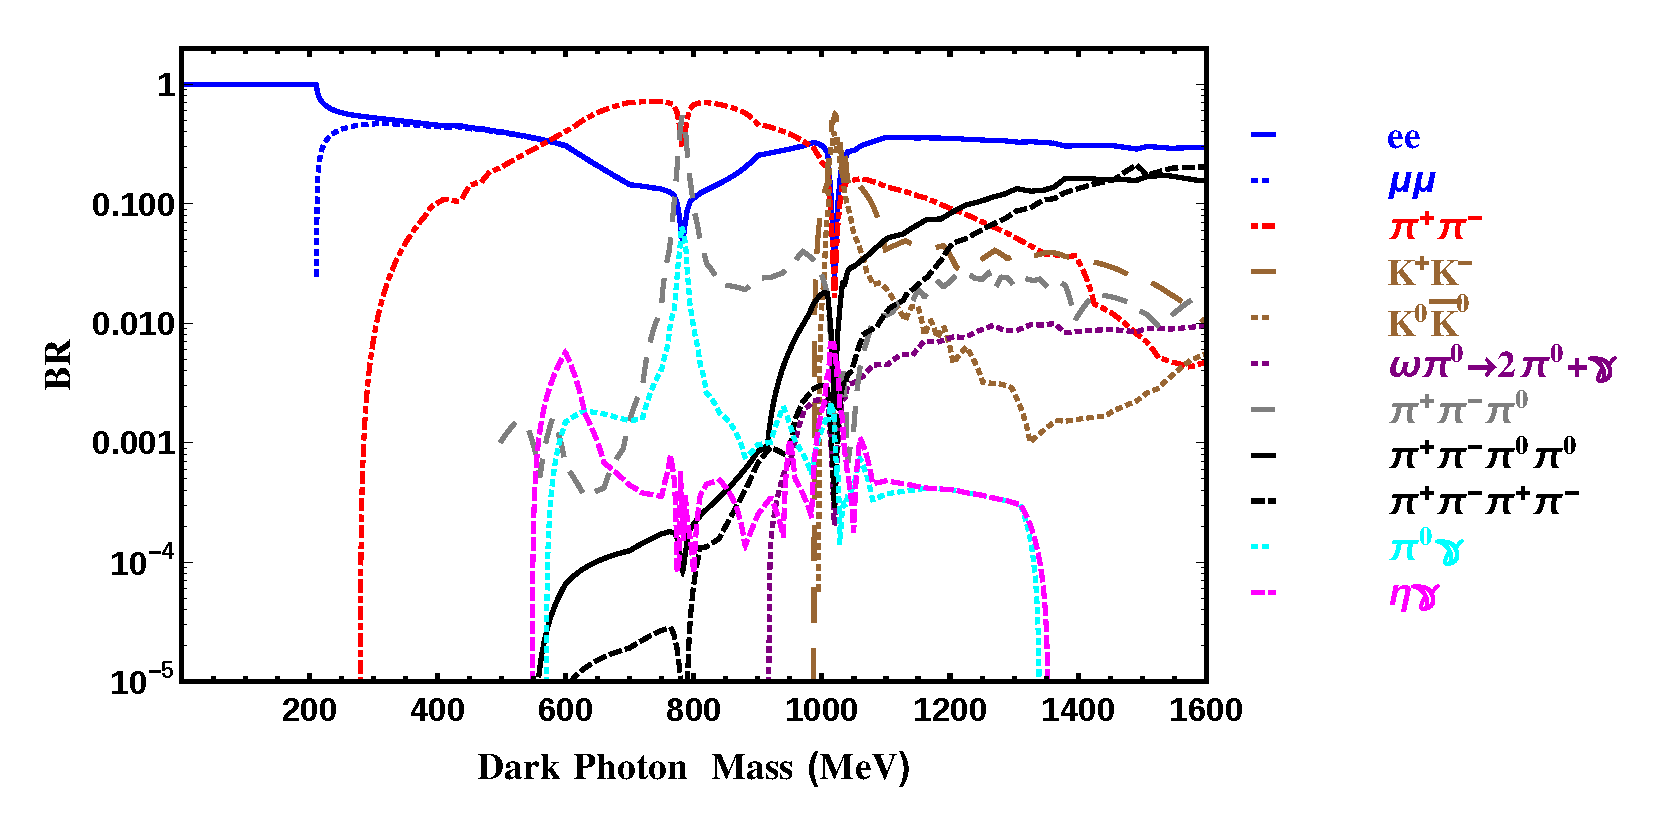
\includegraphics[width=\textwidth]{motivation/figs/darkphoton-BR-1-3000-LOG}
    \caption{Branching ratios for the heavy photon decay to Standard Model particles \cite{liu_signals_2015}.}
    \label{fig:branching}
\end{figure}

In general, the rate of production of a heavy photon with mass $m_{A'}$ is proportional to the rate of the corresponding process for virtual photons, integrated over the mass range bounded by $m_{A'}\pm \frac{\delta m}{2}$.
The kinematics are the same, so the virtual photon process is an irreducible background except that the heavy photon is on-shell and can travel a measurable distance.
A measurement of the virtual photon process can be used to normalize the sensitivity of a search in a data-driven way.
The ratio of differential cross-sections is given in Equation \ref{eq:production}.

\begin{equation}
    \frac{\mathrm{d}\sigma(X \to A' Y \to Z Y)}{\mathrm{d}\sigma(X \to \gamma^* Y \to Z Y)} = \left(\frac{3\pi\epsilon^2}{2N_{eff} \alpha} \right) \left(\frac{m_{A'}}{\delta m} \right)
    \label{eq:production}
\end{equation}

\section{Overview of Searches}
Recent and planned searches for heavy photons can be categorized by the production mechanism, the signature for detection, and the type of facility.

Detection signatures include a mass resonance in the decay products ($e^+e^-$, $\mu^+\mu^-$, or $\pi^+\pi^-$ pairs), missing mass (which allows a search for heavy photons decaying to the dark sector), or displaced vertices.

The common production mechanisms are bremsstrahlung ($e^- Z \to e^- Z A'$), Drell-Yan ($q \bar{q} \to \gamma A'$), $e^+e^-$ annihilation ($e^+e^- \to \gamma A'$), and meson decay ($\pi^0 \to \gamma A'$, $\eta \to \gamma A'$, $\phi \to \eta A'$, and others).
Some experiments look for mass resonances by making all possible pairs (for example, all $\mu^+\mu^-$ pairs) without identifying the production process; these are called ``inclusive'' searches.

Fixed-target experiments and colliders are complementary.
The higher luminosities at fixed-target experiments allow sensitivity at smaller $\epsilon$, particularly for displaced-vertex searches.
Colliders, with their higher center-of-mass energy, can reach larger $m_{A'}$.

\subsection{Beam Dumps}
An electron or proton beam dump will generate heavy photons through bremsstrahlung, Drell-Yan, or meson decays.
If the heavy photon decay length is comparable to the dump length, heavy photons can travel through the dump and decay to visible particles after the dump.
A detector downstream of the dump detects the decay products.


Beam dump experiments have very high luminosities, due to the high currents and thick targets.
Several electron beam dump experiments were run as searches for axion-like or Higgs-like particles, but were reinterpreted to give limits on a heavy photon: E137 \cite{bjorken_search_1988} and E141 \cite{riordan_search_1987} at SLAC, E774 \cite{bross_search_1991} at Fermilab, and an experiment at Orsay \cite{davier_unambiguous_1989}.
Similarly, a proton beam dump experiment at the U70 accelerator was reinterpreted to give limits for heavy photons, both from $\pi^0$ decay and from proton bremsstrahlung \cite{blumlein_new_2014}.

Planned proton beam dump experiments include SHiP at CERN and SeaQuest E1067 at Fermilab.
SHiP is a general-purpose search for dark sector particles \cite{ship_collaboration_facility_2015}; E1067 is an upgrade to an existing dimuon spectrometer to allow parasitic searches for heavy photons \cite{gardner_new_2016}.
NA64 at CERN is an electron beam experiment that uses an electromagnetic calorimeter as an active dump \cite{gninenko_search_2014}.

\subsection{Thin Fixed Targets}
An electron beam incident on a thin target will generate heavy photons through bremsstrahlung, $e^- Z \to e^- Z A'$.
The signature is a mass resonance in the decay products (typically $e^+e^-$; $\mu^+\mu^-$ and $\pi^+\pi^-$ are accessible with beam energies above a couple of GeV).
In contrast to beam dump experiments, these experiments are sensitive to heavy photons that decay promptly, without a resolvable decay length.
The mass resolution can be improved by detecting the recoiling beam electron and/or nucleus.
HPS is the first experiment of this type to attempt a displaced-vertex search.

Two experiments have been run with existing fixed-target spectrometers: one experiment using the A1 spectrometer at MAMI \cite{merkel_search_2014}, and the APEX experiment using the HRS spectrometer at JLab Hall A (a test run was completed, a full run is scheduled) \cite{essig_electron_2011,abrahamyan_search_2011}.
Two experiments are planned: DarkLight at the JLab LERF \cite{balewski_darklight_2014}, and MAGIX at MESA \cite{denig_recent_2016}.

A positron beam incident on a thin target could generate heavy photons through annihilation.
Experiments of this type can detect monophoton final states ($e^+e^- \to \gamma A' \to \gamma \mathrm{dark}$) and identify the heavy photon in the missing mass spectrum. Experiments are proposed at INFN Frascati (PADME \cite{raggi_padme_2015}), VEPP-3 at the Budker Institute at Novosibirsk \cite{wojtsekhowski_searching_2012}.

Proton or ion beams can also be used: the HADES spectrometer was used to measure inclusive $e^+e^-$ pairs from $p$-on-$p$, $p$-on-Nb, and Ar-on-KCl interactions.
The assumed signal was from meson decays \cite{hades_collaboration_searching_2013}.

\subsection{Colliders}
Most collider searches for heavy photons have come from flavor factories, where meson decays are a natural source of heavy photon production.
$e^+e^-$ annihilation or Drell-Yan can also be a significant source of heavy photons.
Displaced-vertex searches are often possible.

Among $e^+e^-$ colliders, BaBar has set limits using $\Upsilon \to \gamma A'$, $A'\to\mu^+\mu^-$ \cite{babar_collaboration_search_2009,soffer_constraints_2014}; KLOE has set limits using $\phi\to \eta A'$ and $e^+e^- \to \gamma A'$ production modes and dielectron, dimuon, and dipion decays \cite{collaboration_search_2012,collaboration_limit_2013,babusci_search_2014,anastasi_limit_2015,collaboration_limit_2016}.
Belle-II is expected to improve on the BaBar result \cite{inguglia_belle_2016}.

$p-p$ colliders have also been used. WASA at COSY looked for $\pi^0 \to \gamma A'$, $A'\to e^+e^-$ \cite{collaboration_search_2013}.
LHCb plans to make a significant impact with a search in $m_{A'}<2m_\mu$ using $D^* \to D^0 A'$, $A'\to e^+e^-$, a search in $m_{A'}>2m_\mu$ using inclusive production and $A'\to \mu^+\mu^-$, and a displaced-vertex search using $\eta \to \gamma A'$, $A'\to \mu^+\mu^-$ \cite{ilten_dark_2015,ilten_inclusive_2016}.

\section{Overview of HPS}

In HPS, the heavy photon is generated through electron bremsstrahlung off of a tungsten nucleus, and detected in its decay to $e^+e^-$.
The process is shown in Figure \ref{fig:ap_prod}.
This process is the analogue of the radiative trident process shown in Figure \ref{fig:tridents_rad}, with a heavy photon substituted for the radiated photon.
Only the $e^+e^-$ pair is triggered on and reconstructed; the recoil electron is typically outside the detector acceptance.
Both the pair invariant mass and vertex position are reconstructed.

\begin{figure}[ht]
    \hspace{5mm}
    \begin{fmffile}{rad1}
        \begin{fmfgraph*}(150,150)
            \fmfstraight 
            \fmfleft{i1,i2,i3,i4}
            \fmfright{o1,o2,o3,o4}
            \fmflabel{$Z$}{i1}
            \fmflabel{$Z$}{o1}
            \fmflabel{$e^-$}{i3}
            \fmflabel{$e^-$}{o2}
            \fmflabel{$e^+$}{o3}
            \fmflabel{$e^-$}{o4}
            \fmf{fermion}{i3,v1,v3,o2}
            \fmf{heavy}{i1,v2,o1}
            \fmf{photon,tension=0,label=$\gamma$}{v1,v2}
            \fmf{fermion}{o3,v4,o4}
            \fmf{photon,tension=2,label=$A'$}{v3,v4}
        \end{fmfgraph*}
    \end{fmffile}
    \hspace{10mm}
    \begin{fmffile}{ap2}
        \begin{fmfgraph*}(150,150)
            \fmfstraight 
            \fmfleft{i1,i2,i3,i4}
            \fmfright{o1,o2,o3,o4}
            \fmflabel{$Z$}{i1}
            \fmflabel{$Z$}{o1}
            \fmflabel{$e^-$}{i3}
            \fmflabel{$e^-$}{o2}
            \fmflabel{$e^+$}{o3}
            \fmflabel{$e^-$}{o4}
            \fmf{fermion}{i3,v1,v3,o2}
            \fmf{heavy}{i1,v2,o1}
            \fmf{fermion}{o3,v4,o4}
            \fmf{photon,tension=2,label=$\gamma$}{v1,v4}
            \fmffreeze
            \fmf{photon,tension=0,label=$A'$}{v3,v2}
        \end{fmfgraph*}
    \end{fmffile}
    \hspace{5mm}
    \caption{Heavy photon production and decay. The heavy photon ($A'$) is on-shell, and can travel some distance before decaying in free space.}
    \label{fig:ap_prod}
\end{figure}

Two analyses are performed on the same data set.
A pure bump-hunt search at large $\epsilon$ assumes the heavy photon decays at the target, which improves the mass resolution.
This is a search for a mass resonance, using only the pair invariant mass; it is described fully in \cite{moreno_search_2016}.
A displaced-vertex search at small $\epsilon$ rejects pairs originating from the target.
Because the heavy photon must travel a measurable distance, this search is not sensitive to large $\epsilon$.

This dissertation presents the displaced-vertex search.

\subsection{Signal Kinematics}
The kinematics of heavy photon production can be calculated using the Weizs{\"a}cker-Williams approximation (where the nucleus is replaced by an effective photon flux); this is done in \cite{bjorken_new_2009}, based on work in \cite{tsai_pair_1974,tsai_axion_1986}.
An exact (to leading order, with radiative corrections) calculation shows similar results \cite{beranek_theoretical_2013,beranek_study_2014}
The differential cross-section for an electron with energy $E_0$ to produce a heavy photon with energy $E_{A'}=xE_0$, at angle $\theta_{A'}$ from the beam (in the lab frame), is
\begin{equation}
    \frac{\mathrm{d}\sigma}{\mathrm{d}x \mathrm{d}\cos \theta_{A'}} \approx \frac{8 Z^2 \alpha^3\epsilon^2E_0^2}{U^2} \frac{\chi}{Z^2} \left( 1-x+\frac{x^2}{2} - \frac{x(1-x)m^2_{A'} (E_0^2 x \theta_{A'}^2)}{U^2} \right)
    \label{eq:cx_xtheta}
\end{equation}
where $\chi/Z^2$ ($\sim 5-10$ for values of $m_{A'}<100$ MeV, where HPS is sensitive) depends on atomic form factors and kinematics, and $U(x,\theta_{A'}) = E_0^2x\theta_{A'}^2 + m_{A'}^2\frac{1-x}{x} + m_e^2 x$ is the virtuality of the electron in the intermediate state.
The approximation assumes $m_e \ll m_{A'} \ll E_0$ and $x\theta_{A'}^2 \ll 1$.
The characteristic angle of emission is set by $U(x,\theta_{A'})-U(x,0)\sim U(x,0)$, which occurs at $\theta_{A'}\sim \frac{m_{A'}\sqrt{1-x}}{xE_0}$.

Integrating out $\theta_{A'}$ and ignoring $m_e$, the differential cross-section is
\begin{equation}
    \frac{\mathrm{d}\sigma}{\mathrm{d}x} \approx \frac{8 Z^2 \alpha^3\epsilon^2 x}{m_{A'}^2} \frac{\chi}{Z^2} \left( 1 + \frac{x^2}{3(1-x)} \right)
    \label{eq:cx_x}
\end{equation}
There is a cutoff at $1-x = \max \left(\frac{m_e^2}{m_{A'}^2},\frac{m_{A'}^2}{E_0^2} \right)$, and the median value of $1-x$ is $\max \left(\frac{m_e}{m_{A'}},\frac{m_{A'}}{E_0} \right)$.

The overall rate is controlled by $\frac{\alpha^3\epsilon^2}{m_{A'}^2}$, so heavy photon production is increasingly less likely at larger $m_{A'}$.
From Equation \ref{eq:cx_x}, the heavy photon typically takes most of the incident electron's momentum: $E_{A'}\approx E_0$.
This means that the typical opening angle of the decay products is $2m_{A'}/E_0$, and the typical vertex displacement is
\begin{equation}
    \gamma c\tau \approx \frac{3\hbar E_0}{N_{eff}m_{A'}^2\alpha\epsilon^2 c}
\end{equation}
From Equation \ref{eq:cx_xtheta}, $\theta_{A'}$ is dominated by small values: the typical value of $\theta_{A'}$ is $\left(\frac{m_{A'}}{E_0}\right)^{3/2}$, so $\theta_{A'}$ is smaller than the opening angle of the decay products and it is a good approximation to assume the heavy photon is emitted in the beam direction.

The recoiling incident electron is soft and also largely balances the $p_\perp$ of the heavy photon, and therefore is at relatively wide angle $\theta_R\sim \sqrt{\frac{m_{A'}}{E_0}}$.
It rarely makes it through the full length of the detector, and is not easily tracked.

\subsection{Physics Backgrounds}
The major sources of $e^+e^-$ backgrounds are radiative tridents, Bethe-Heitler tridents, and pair conversions of wide-angle bremsstrahlung photons.

As discussed in Section \ref{sec:signatures}, the radiative trident and heavy photon processes have the same kinematics.
The radiative trident process is therefore an irreducible background, except that heavy photons can be distinguished by the mass resonance and measurable decay length.

\begin{figure}[ht]
    \hspace{5mm}
    \begin{fmffile}{rad1}
        \begin{fmfgraph*}(150,150)
            \fmfstraight 
            \fmfleft{i1,i2,i3,i4}
            \fmfright{o1,o2,o3,o4}
            \fmflabel{$Z$}{i1}
            \fmflabel{$Z$}{o1}
            \fmflabel{$e^-$}{i3}
            \fmflabel{$e^-$}{o2}
            \fmflabel{$e^+$}{o3}
            \fmflabel{$e^-$}{o4}
            \fmf{fermion}{i3,v1,v3,o2}
            \fmf{heavy}{i1,v2,o1}
            \fmf{photon,tension=0,label=$\gamma$}{v1,v2}
            \fmf{fermion}{o3,v4,o4}
            \fmf{photon,tension=2,label=$\gamma$}{v3,v4}
        \end{fmfgraph*}
    \end{fmffile}
    \hspace{10mm}
    \begin{fmffile}{rad2}
        \begin{fmfgraph*}(150,150)
            \fmfstraight 
            \fmfleft{i1,i2,i3,i4}
            \fmfright{o1,o2,o3,o4}
            \fmflabel{$Z$}{i1}
            \fmflabel{$Z$}{o1}
            \fmflabel{$e^-$}{i3}
            \fmflabel{$e^-$}{o2}
            \fmflabel{$e^+$}{o3}
            \fmflabel{$e^-$}{o4}
            \fmf{fermion}{i3,v1,v3,o2}
            \fmf{heavy}{i1,v2,o1}
            \fmf{fermion}{o3,v4,o4}
            \fmf{photon,tension=2,label=$\gamma$}{v1,v4}
            \fmffreeze
            \fmf{photon,tension=0,label=$\gamma$}{v3,v2}
        \end{fmfgraph*}
    \end{fmffile}
    \hspace{5mm}
    \caption{Radiative trident diagrams.}
    \label{fig:tridents_rad}
\end{figure}

The Bethe-Heitler trident process (Figure \ref{fig:tridents_bh}), and its interference with the radiative trident process, is another background.
In contrast to heavy photons and radiative tridents, pairs from non-radiative tridents are not peaked at high $x$.
In general, the two electrons are not distinguishable and either $e^+e^-$ pair is a potential background.

\begin{figure}[ht]
    \hspace{5mm}
    \begin{fmffile}{bh1}
        \begin{fmfgraph*}(150,150)
            \fmfstraight 
            \fmfleft{i1,i2,i3,i4}
            \fmfright{o1,o2,o3,o4}
            \fmflabel{$Z$}{i1}
            \fmflabel{$Z$}{o1}
            \fmflabel{$e^-$}{i4}
            \fmflabel{$e^-$}{o2}
            \fmflabel{$e^+$}{o3}
            \fmflabel{$e^-$}{o4}
            \fmf{fermion}{i4,v1,o4}
            \fmf{heavy}{i1,v2,o1}
            \fmffreeze
            \fmf{photon,tension=1,label=$\gamma$}{v1,v3}
            \fmf{photon,tension=1,label=$\gamma$}{v2,v4}
            \fmf{fermion}{o2,v4,v3,o3}
        \end{fmfgraph*}
    \end{fmffile}
    \hspace{10mm}
    \begin{fmffile}{bh2}
        \begin{fmfgraph*}(150,150)
            \fmfstraight 
            \fmfleft{i1,i2,i3,i4}
            \fmfright{o1,o2,o3,o4}
            \fmflabel{$Z$}{i1}
            \fmflabel{$Z$}{o1}
            \fmflabel{$e^-$}{i4}
            \fmflabel{$e^-$}{o2}
            \fmflabel{$e^+$}{o3}
            \fmflabel{$e^-$}{o4}
            \fmf{fermion}{i4,v1,o4}
            \fmf{heavy}{i1,v2,o1}
            \fmffreeze
            \fmf{photon,tension=2,label=$\gamma$}{v1,v3}
            \fmf{photon,tension=2,label=$\gamma$}{v2,v4}
            \fmf{fermion}{o2,v3,v4,o3}
        \end{fmfgraph*}
    \end{fmffile}
    \hspace{5mm}
    \caption{Bethe-Heitler trident diagrams.}
    \label{fig:tridents_bh}
\end{figure}

Wide-angle bremsstrahlung (where the photon and electron are both at large angles from the beam axis), followed by pair conversion of the photon (either in the target or in the first parts of the detector), is another significant background.
Since the photon is on-shell, the $e^+e^-$ pair from the pair conversion is generally not in the HPS acceptance.
However, the scattered incident electron and the positron from the pair conversion are often in the acceptance.
